\chapter{安全链路系统设计与实现}
本章节主要介绍安全链路系统的整体设计与具体实现,
首先介绍安全链路系统的整体设计,并对其特点进行简要分析。
然后分别从入口节点、中继节点、出口节点三个组成部分介绍系统实现、系统配置、系统功能和系统分析。

\section{系统框架}
安全链路系统由入口、中继和出口节点三部分组成,其中入口节点作为客户端,多个中继节点进行流量的转发,出口节点将与真实互联网进行交互。
系统设计用一个UUID标识一条链路,流量在转发时会根据配置的信息根据得到的UUID进行相应转发。

安全链路系统有三个组成部分:入口节点、中继节点、出口节点。
\begin{itemize}
  \item \textbf{入口节点}:入口节点(客户端程序)处在整个加密安全链路系统的起始部分,运行在用户本地,负责作为HTTP代理或者SOCKS5代理将本地流量通过加密隧道传输到目的服务器。
  \item \textbf{中继节点}:中继节点处在整个加密安全链路系统的中心部分,负责将入口节点的流量转发到出口节点,通常一条完整的加密隧道可以包含多个中继节点。
  \item \textbf{出口节点}:出口节点处于整个加密安全链路系统的边缘部分,负责接收来自中继节点的连接,并与目标服务器通信。
\end{itemize}

\begin{figure}[H]
  \centering
  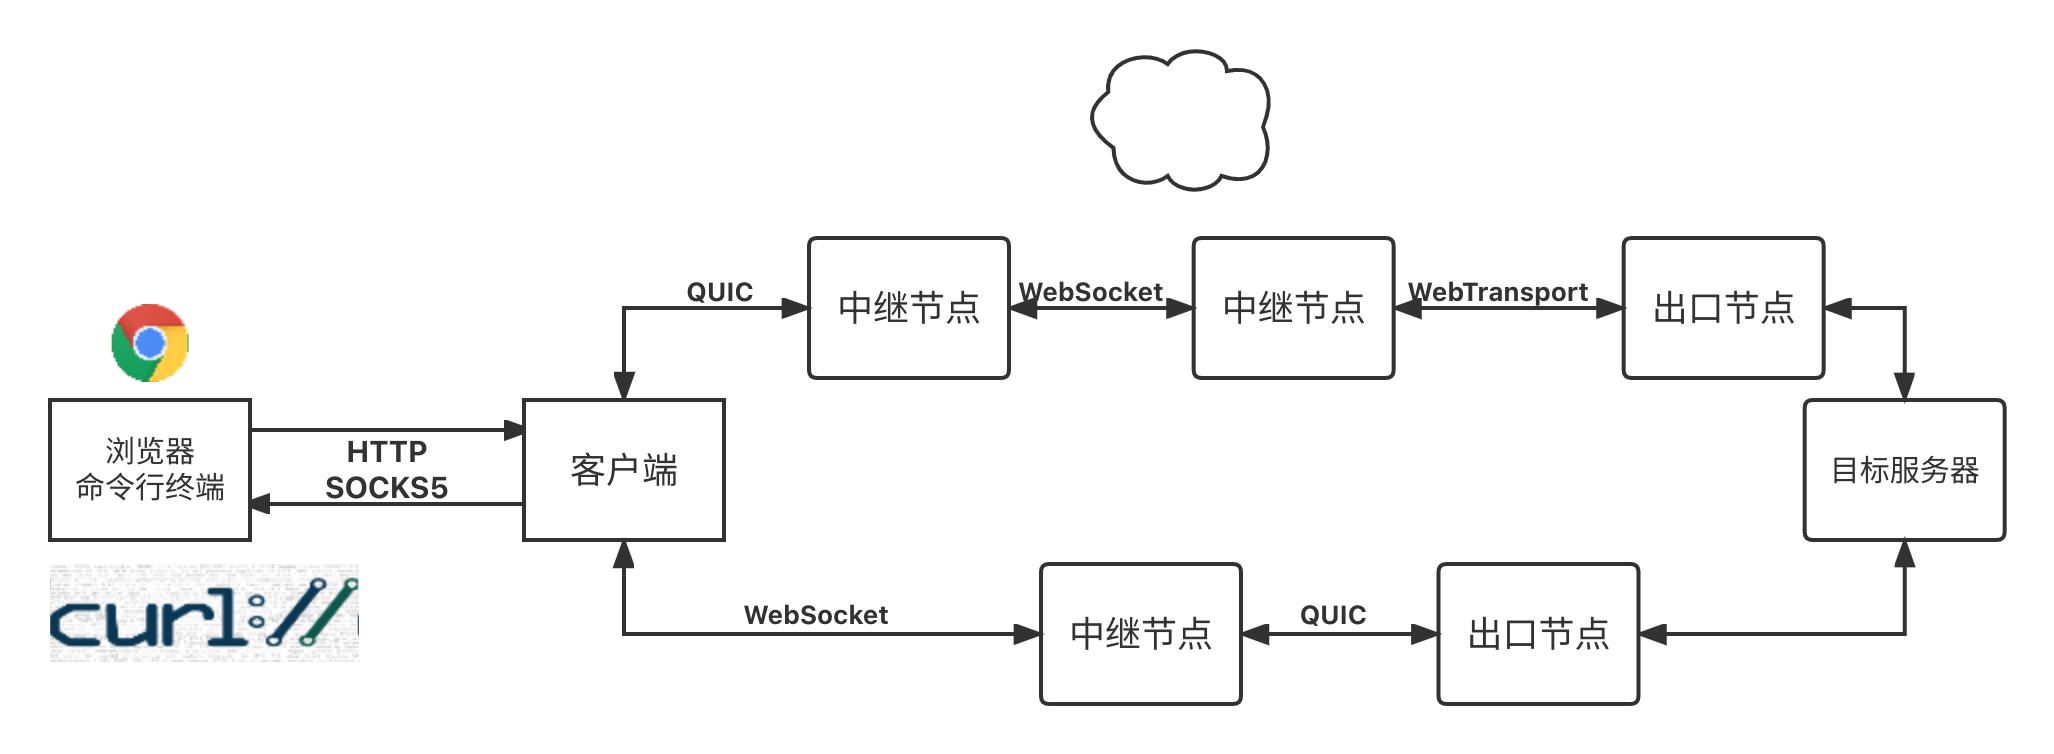
\includegraphics[width=\textwidth]{masky}
  \caption{一种对抗中间人流量分析的安全链路}
\end{figure}

\subsection{加密隧道}
通用唯一标识符(英语:Universally Unique Identifier,缩写:UUID)是用于计算机体系中以识别信息的一个128位标识符。
UUID具有唯一性,重复UUID码概率接近零,可以忽略不计。
安全链路系统通过一个UUID表示一个加密隧道,数据报文在链路传输中会通过UUID找到下一跳的节点,如果没有发现符合的UUID会断开连接。

安全链路系统支持3种加密传输协议,分别是QUIC、WebSocket和WebTransport。
如果传输协议是WebSocket和WebTransport,UUID作为初始HTTP请求的URL中的秘密,所有访问秘密URL的请求代理到下一跳节点,而其他的HTTP请求返回正常的HTTP响应。
如果传输协议是QUIC,发送节点向下一个节点传输数据时,会在第一个数据报文头部填充隧道对应的UUID。接收节点会解密前16字节的UUID进行验证,并根据UUID对应的隧道找到下一跳节点。
此外,加密隧道中相邻节点支持使用不同的加密传输协议,入口节点每次会随机选择一条加密隧道传输数据,因此增加了反追踪的能力。

\subsection{系统配置}
系统选用YAML作为系统配置格式,每一个节点(入口节点、中继节点和出口节点)都有一个对应的配置文件,
包含连接的链路信息、本地端口、日志记录级别等信息。

\section{特点分析}
\subsection{安全性}
对于发送者而言,接收者的出口节点正是其入口节点。
由于接收者和发送者的IP地址在任何中继中都不是通过明文传输,所以若有人在中继路径中的任何一点窃听,都无法同时识别两端。
数据包在链路传输中通过加密协议(QUIC、WebSocket、WebTransport)加密,这些协议使用TLS1.3,保证了认证加密(authenticated encryption)安全。

\subsection{匿名性}
加密通信隧道会对包括下一个节点的IP地址在内的数据,进行多次加密,在出口节点将其提交。
每个中继都会对一层加密的数据进行解密,以知道数据的下一个发送目的地,然后将剩余的加密数据发送给它。
最后的中继会解密最内层的加密数据,并在不会泄露或得知源IP地址的情况下,将原始数据发送至目标地址。

\subsection{便携性}
整个安全链路系统主要通过Go语言实现,支持二进制代码的跨平台软件开发,可以从一个开发主机为多个平台编译代码。
并且,目前对实现的客户端、中继节点、出口节点都通过Docker都实现了对应用程序的打包,并且提交到Docker Hub上。
这有助于实现灵活性和便携性,应用程序在任何Linux服务器上都可以执行。


\section{入口节点}
入口节点(客户端)运行在用户本地端口,负责作为HTTP代理或者SOCKS5代理将本地流量通过加密隧道传输到目的服务器。
本节具体介绍出口节点系统设计,以及其包含的主要功能。

\subsection{系统实现}
入口节点(客户端)系统通过Go语言实现,默认在本地1080端口同时作为HTTP代理和SOCKS5代理,在本地1081端口运行Web控制页面和Web API。
如果客户端接收需要转发的流量,会首先查看数据流的第一个字节,如果是5将其作为SOCKS5代理处理,否则作为HTTP代理处理。
程序运行时,客户端会根据选择的模式选择是否对流量进行代理。
如果选择代理流量,每次会随机选择配置文件中一条加密的隧道中继流量,用户还可以在Web控制端固定选择一条加密隧道。

\subsection{系统配置}
入口节点(客户端)系统采用YMAL作为配置文件格式,如下是入口节点的相关配置信息和一个示例配置YAML文件:
\begin{table}[H]
  \begin{tabular}{| m{10em} | m{24em} |}
  \hline
  端口号(port) & 客户端在本地监听的端口,应用程序可以通过设置HTTP代理或者SOKCS5代理为这个本地端口实现流量通过隧道加密发送到目的地。  \\ \hline
  模式(mode)  & 客户端支持的数据包路由模式,有直连(Direct)、规则(Rule)、代理(Global)三种模式。直连(Direct):直接将数据包转发到互联网。规则(Rule):基于规则的数据包路由。代理(Global):所有数据包将通过加密隧道转发到目的地。\\ \hline            
  允许局域网连接(allowLan)  & 是否允许本地网络连接,设置为true以允许从其他局域网IP地址与本地客户端建立连接,否则不允许。如果允许本地连接,客户端程序监听在0.0.0.0,否则监听在127.0.0.1。 \\ \hline         
  日志等级(logLevel)  & 日志记录的等级,分为信息(info)、警告(warn)、错误(error)三种级别,通过设置不同的日志等级可以控制命令行输出日志。 \\ \hline    
  代理(proxies)  & 客户端支持的多条加密隧道 \\ \hline              
  \end{tabular}
  \caption{入口节点相关配置信息}
\end{table}

\begin{table}[H]
  \begin{tabular}{| m{10em} | m{22em} |}
  \hline
  id & 一个随机生成的UUID,用于标识隧道,同时作为隧道中节点的共享秘密。  \\ \hline
  name  & 一条隧道的名称,用于表示隧道的相关信息。 \\ \hline            
  type  & 客户端到下一个中继节点的传输协议,包括quic、websocket、webtransport三种传输协议。 \\ \hline    
  server  & 加密隧道要经过的各个节点的地址,如果传输协议是quic则为一个ip地址和端口号的组合,否则为一个域名。 \\ \hline              
  \end{tabular}
  \caption{代理(proxies)表示客户端支持的多条加密隧道,每个隧道包含的信息。}
\end{table}

\begin{figure}[H]
  \centering
  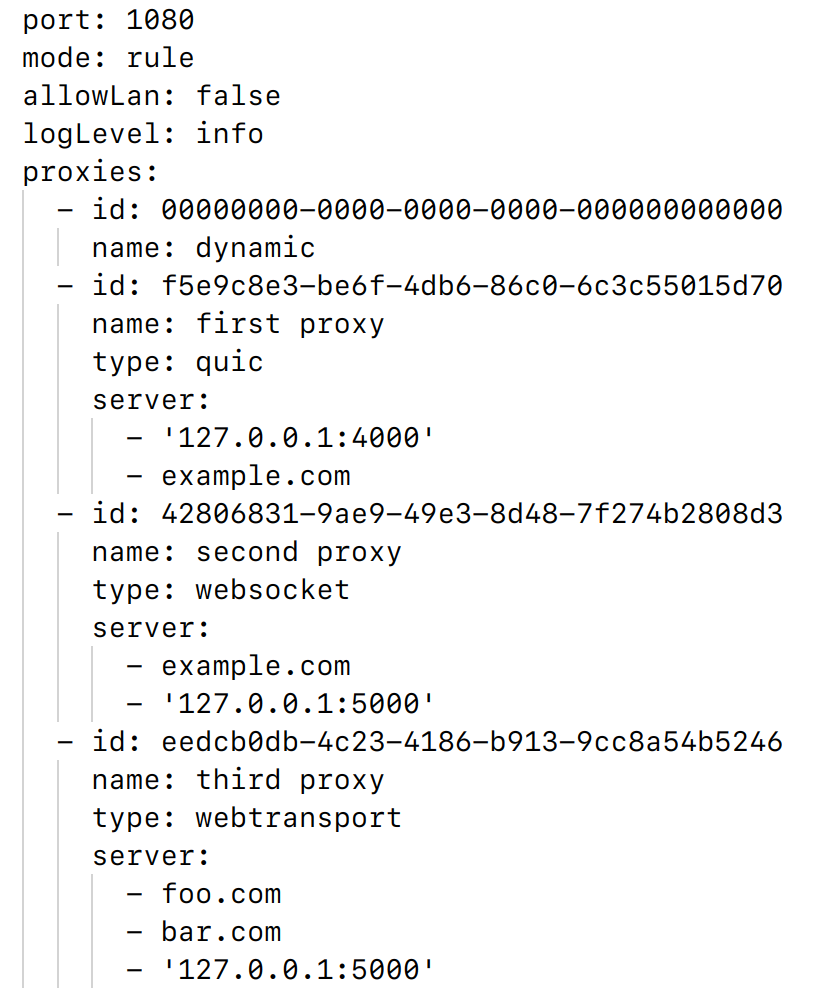
\includegraphics[width=\textwidth]{client}
  \caption{一个入口节点(客户端)示例配置文件}
\end{figure}

\subsection{系统功能}
\textbf{代理流量:}
通过设置使用代理(HTTP或SOCKS5)为安全链路客户端,用户的流量请求通过加密隧道发送到目标服务器。

\textbf{网页控制:}
客户端实现了一个简单的Web页面,默认运行在本地http://127.0.0.1:1081。
用户可以通过GUI修改配置,查看当前连接信息和系统运行日志等,还可以主动选择不同的加密隧道进行连接。

\begin{figure}[H]
  \centering
  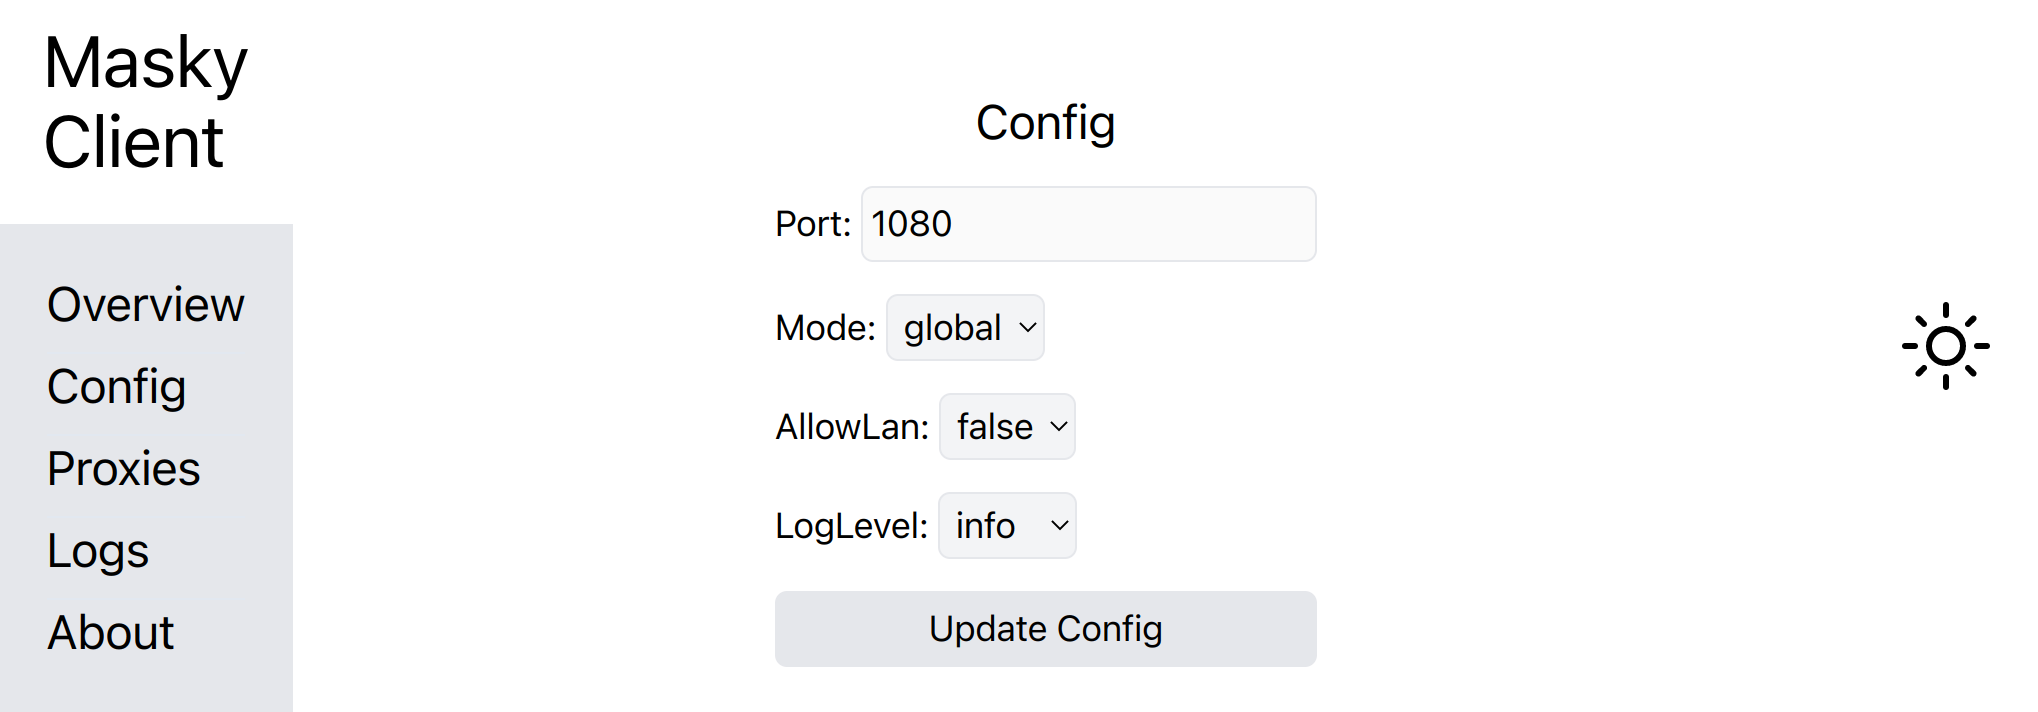
\includegraphics[width=\textwidth]{client_web}
  \caption{控制客户端的简单的Web页面}
\end{figure}

\textbf{API控制:}
目前初步设计完成了程序的RESTful API,程序在运行的同时会在一个端口运行API服务器。
在不重启程序的前提下,可以通过访问API接口获取程序运行的一些信息,同时也能控制程序内部的配置。
基于API,程序运行时会在同一个端口运行静态网页服务器,用户可以通过浏览器打开相应页面,通过GUI完成API接口的功能。

\textbf{IP匹配:}
客户端可执行程序包括一个IP数据库,来源于免费的IP地理定位数据库Geolite2。
如果选择规则模式,通过geolite2数据库得到IP地址对应的国家isocode,然后根据设置作出直连或者代理的选择。
域名和isocode用map存储,并且用一个读写锁保护,允许并发读操作,每次只允许一个写操作。
每次查询域名,如果map命中直接返回对应isocode,否则通过数据库查询并更新map。

\textbf{链路选择:}
链路选择支持静态链路和动态链路。安全链路提供一个链路池,用户可以根据需求自行设置想要的传输方式。
\begin{itemize}
  \item \textbf{静态链路}:选择客户端配置文件中一条特定的加密传输链路,所有流量都会通过这条加密隧道传输到目的服务器。
  \item \textbf{动态链路}:如果客户端配置文件包含多个加密传输链路,每次会随机选择一条加密隧道传输数据。
\end{itemize}

\subsection{系统分析}
\textbf{安全性:}
如果选择规则模式,流量会根据基于isocode匹配路由到不同的目的位置。
并且客户端的配置可以包含多个加密隧道,每次会随机选择一条加密隧道传输数据报文,这提高了整个链路系统的安全性。

\textbf{匿名性:}
如果选择动态链路,由于每次随机选择一条链路,并且每条链路都包含多个中继节点,因此攻击者难以确定加密隧道的起始和终点IP地址,提高了整个链路系统的匿名性。

\textbf{便捷性:}
客户端支持三种方式修改配置:直接修改对应的YAML配置文件相应的内容、调用API接口更改配置、通过Web页面修改配置。

客户端支持三种模式选择:直连(Direct):直接将数据包转发到互联网,规则(Rule):基于规则的数据包路由,代理(Global):所有数据包将通过加密隧道转发到目的地。

客户端可执行程序包括一个Geolite2国家IP数据库,可以得到某一IP对应的国家isocode,默认被用于基于规则的路由匹配上。

\section{中继节点}
中继节点处在整个加密安全链路系统的中心部分,负责将入口节点的流量转发到出口节点,通常一条完整的加密隧道可以包含多个中继节点。
本节具体介绍中继节点系统设计,以及其包含的主要功能。

\subsection{系统实现}
中继节点系统通过Go语言实现,首先验证连接的UUID,根据配置和隧道对应UUID找到下一跳节点。
如果中继节点的传输协议是QUIC,那么中继节点暴露在网络上,在一个端口监听来自加密隧道的上一个节点的连接。
如果中继节点的传输协议是WebSocket或WebTransport,中继节点可以隐藏在一个反向代理服务器(如Nginx)后面,当访问特定的URL(标识隧道的UUID)才能建立连接。

\subsection{系统配置}
中继节点系统采用YMAL作为配置文件格式,如下是中继节点的相关配置信息和一个示例配置YAML文件:

\begin{table}[H]
  \begin{tabular}{| m{10em} | m{24em} |}
  \hline
  端口号(port) & 中继节点在本地监听的端口。  \\ \hline
  端口号(type) & 中继节点支持的的传输协议,包括quic、websocket、webtransport三种传输协议。  \\ \hline
  证书(cert) & 由CA签发的证书。  \\ \hline
  私钥(key) & 证书对应的私钥。  \\ \hline
  日志等级(logLevel)  & 日志记录的等级,分为信息(info)、警告(warn)、错误(error)三种级别,通过设置不同的日志等级可以控制命令行输出日志。 \\ \hline    
  代理(proxies)  & 中继节点支持的多条加密隧道。 \\ \hline              
  \end{tabular}
  \caption{中继节点相关配置信息}
\end{table}

\begin{table}[H]
  \begin{tabular}{| m{10em} | m{22em} |}
  \hline
  id & 一个随机生成的UUID,用于标识隧道,同时作为隧道中节点的共享秘密。  \\ \hline        
  type  & 中继节点到下一个节点(中继节点或出口节点)的传输协议,包括quic、websocket、webtransport三种传输协议。 \\ \hline    
  server  & 中继节点的下一个节点(中继节点或出口节点)的地址,如果传输协议是quic则为一个ip地址和端口号的组合,否则为一个域名。 \\ \hline              
  \end{tabular}
  \caption{代理(proxies)表示中继节点支持的多条加密隧道,每个隧道包含的信息。}
\end{table}

\begin{figure}[H]
  \centering
  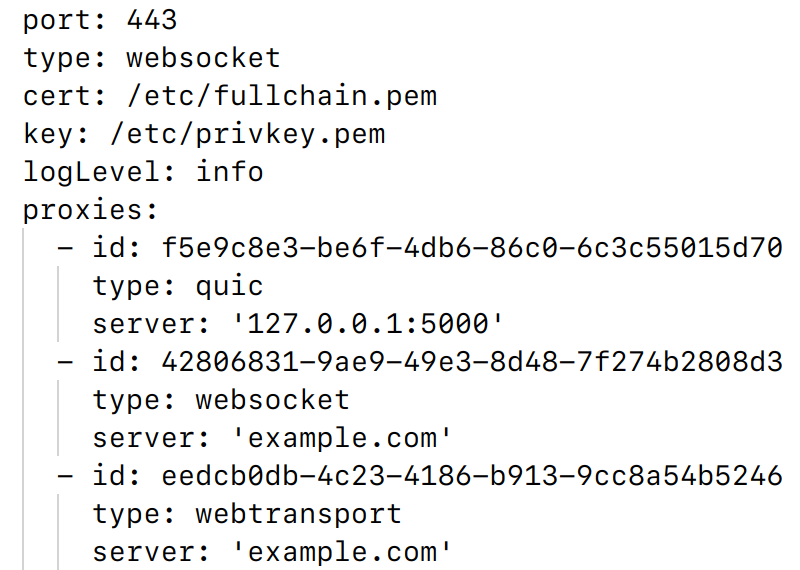
\includegraphics[width=\textwidth]{relay}
  \caption{一个中继节点示例配置文件}
\end{figure}

\subsection{系统功能}

\textbf{中继流量:}
中继节点接受来自客户端节点或者中继节点的连接,将加密流量转发到隧道的下一个节点(中继节点或者出口节点)。
一条加密隧道的中继节点可以有多个,保证了难以追踪入口节点的IP地址。

\textbf{身份认证:}
每一个中继节点的配置文件包括支持的加密隧道信息,其中每个加密隧道只包括标识隧道的UUID和隧道的下一个节点(中继节点或出口节点)。
当中继节点接收来自其他节点的连接,会首先验证发送的UUID包含在配置文件的加密隧道中,如果验证通过则中继流量到对应隧道的下一个节点,否则会返回一个正常的Web页面或者404(当传输协议是WebSocket或WebTransport)。

\subsection{系统分析}

\textbf{安全性:}
出口节点只接受信任的中继节点的连接,对于不符合配置的IP的连接不响应,并验证连接的UUID是否正确。
出口节点解密报文信息,得到真正目的地址,然后与目的服务器建立连接,将解密后的数据报文发送到目的服务器。
一条加密隧道可以包含多个中继节点,攻击者窃听流量不知道流量的源客户端IP地址和目的服务器IP地址,保证了链路系统的安全性。

\textbf{匿名性:}
一条加密隧道可以包含多个中继节点,每个中继节点只负责中继加密流量到一个节点,除此之外不知道任何信息。
对于一个加密隧道的一个中继节点,其只知道上一个节点(不知道是中继节点还是入口节点)的IP地址和下一个节点(不知道是中继节点还是出口节点)的IP地址,这提高了整个链路系统的匿名性。

\section{出口节点}
出口节点处于整个加密安全链路系统的边缘,负责接收来自中继节点的连接,并与目标服务器通信。
本节具体介绍出口节点系统设计,以及其包含的主要功能。

\subsection{系统实现}
出口节点系统通过Go语言实现,首先验证连接的UUID,如果验证正确与目标服务器建立连接。
基于WebSocket/WebTransport的加密隧道出口节点可以隐藏在已有的Web服务器(如Nginx、Caddy等)下。

\begin{figure}[H]
  \centering
  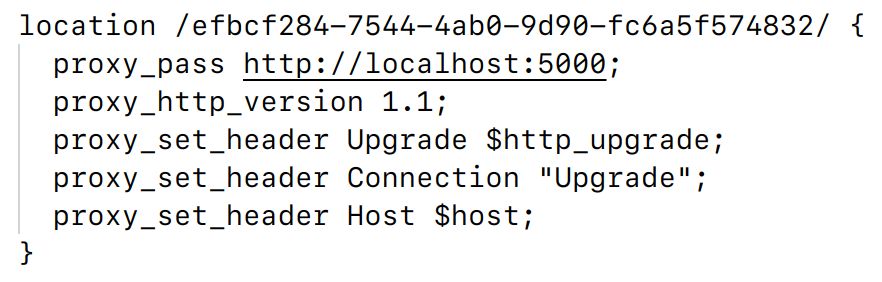
\includegraphics[width=\textwidth]{nginx}
  \caption{基于WebSocket的加密隧道:用Nginx作为反向代理,秘密URL为efbcf284-7544-4ab0-9d90-fc6a5f574832,出口节点运行在本地端口5000,相应的Nginx配置}
\end{figure}

\subsection{系统配置}
出口节点系统采用YMAL作为配置文件格式,如下是出口节点的相关配置信息和一个示例配置YAML文件:
\begin{table}[H]
  \begin{tabular}{| m{10em} | m{22em} |}
  \hline
  端口号(port) & 出口节点在本地监听的端口。  \\ \hline
  端口号(type) & 出口节点支持的的传输协议,包括quic、websocket、webtransport三种传输协议。  \\ \hline
  证书(cert) & 由CA签发的证书。  \\ \hline
  私钥(key) & 证书对应的私钥。  \\ \hline
  日志等级(logLevel)  & 日志记录的等级,分为信息(info)、警告(warn)、错误(error)三种级别,通过设置不同的日志等级可以控制命令行输出日志。 \\ \hline       
  代理(proxies)  & 出口节点支持的多条加密隧道。 \\ \hline                
  \end{tabular}
  \caption{出口节点相关配置信息}
\end{table}

\begin{table}[H]
  \begin{tabular}{| m{10em} | m{22em} |}
  \hline
  id & 一个随机生成的UUID,用于标识隧道,同时作为隧道中节点的共享秘密。  \\ \hline                  
  \end{tabular}
  \caption{代理(proxies)表示出口节点支持的多条加密隧道,每个隧道包含的信息。}
\end{table}

\begin{figure}[H]
  \centering
  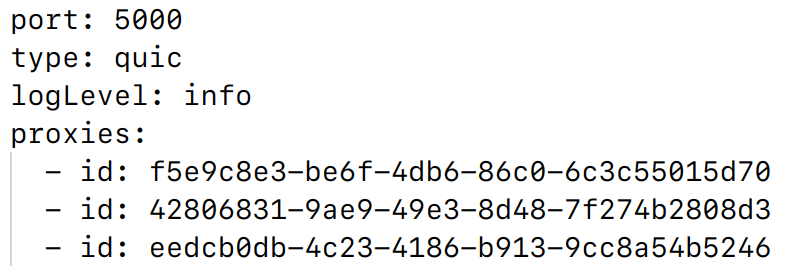
\includegraphics[width=\textwidth]{exit}
  \caption{一个出口节点示例配置文件}
\end{figure}

\subsection{系统功能}

\textbf{中继流量:}
出口节点接收来自上一个中继节点的加密数据报文,解密后发送到原本的目的地址。
从目标服务器的角度而言,出口节点是与其直接进行通信的入口节点。

\textbf{身份认证:}
每一个出口节点的配置文件包括支持的加密隧道信息,其中每个加密隧道只包括标识隧道的UUID。
当出口节点接收来自其他节点的连接,会首先验证发送的UUID包含在配置文件的加密隧道中,如果验证通过则中继流量到目的地,否则会返回一个正常的Web页面或者404(当传输协议是WebSocket或WebTransport)。

\subsection{系统分析}

\textbf{安全性:}
出口节点只接受信任的中继节点的连接,对于不符合配置的IP的连接不响应,并验证连接的UUID是否正确。
出口节点解密报文信息,得到真正目的地址,然后与目的服务器建立连接,将解密后的数据报文发送到目的服务器。

\textbf{匿名性:}
虽然出口节点知道用户要访问的服务,但不知道用户的源IP地址,只知道上一个中继节点的IP地址,因此保证了安全链路的匿名性。
